\chapter{Theoretical background and state-of-the-art}
\label{cha:intro}


In this chapter theory behind computer vision, 3D reconstruction and mathematical apparatus used in our algorithm are introduced. Pinhole camera model and basics of stereo and mono vision are briefly discussed. Other topics -- Difference of Gaussians edge detection and 3D rotation conventions -- can be found in Appendices B and C, respectively. Literature connected with this topic is overviewed. Finally, \textit{Rebvo} \cite{jose2015realtime} algorithm flow  is described.

%-----------------

\section{Pinhole camera model}
\label{sec:pinhole}

Pinhole camera model \cite{hartley2003multiple} is a widely used \cite{straight} and simple model that establishes connection between world coordinates $\Re^3$ and image-domain coordinates $\Re^2$ (i.e. projective geometry).

\begin{figure}[ht]
	\centering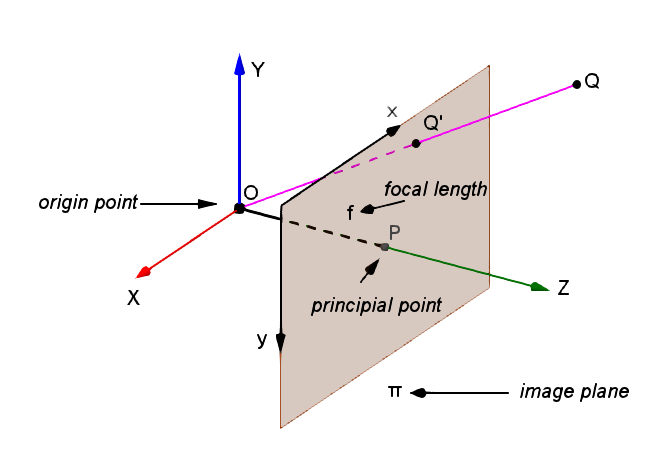
\includegraphics[width=0.8\linewidth]{img/projective.PNG}
	\caption{Image formation in pinhole camera model. Source: \cite{szczesny}}
	\label{fig:projective}
\end{figure}

Operation of pinhole camera is depicted in Fig.~\ref{fig:projective}. Every 3D point $Q$ can be associated with a ray $QO$ that passes through camera origin $O$, which in the simplest case can be defined as origin of the 3D coordinate system origin. Such ray can be defined with homogeneous coordinates as set of points $\{(X, Y, Z)\}$ that satisfy Eq.~\ref{eq:homo}:


\begin{equation}
(X, Y, Z) = k(Q_x, Q_y, Q_z)
\label{eq:homo}
\end{equation}
where:
\begin{eqwhere}[2cm]
	\item[$k$] real parameter, \(k \neq 0\),
	\item[$Q$] world coordinates point.
\end{eqwhere}

Image plane \(\pi\) is a rectangle parallel to plane \(XOY\). Its distance from origin is equal to \(f\) (focal length). Usually it is assumed that image plane's \(z\) coordinate is positive -- otherwise formed image would be upside down. Point where axis \(OZ\) intersects \(\pi\) is called principal point.

World coordinate points Q are projected onto \(\pi\) as \(Q'\), thus forming a 2D image. This relationship can be concisely written using camera matrix as in Eq.~\ref{eq:camera}.

\begin{equation}
q = Q' \sim \underbrace{ \underbrace{  \begin{bmatrix}
		f_{x} & s & c_{x} \\ 
		0 & f_{y} & c_{y} \\ 
		0 & 0 & 1
	\end{bmatrix}
}_{K} R \left [ I | -t \right ] }_{C} Q
\label{eq:camera}
\end{equation}
where:
\begin{eqwhere}[2cm]
	\item[$q$] 2D point on image plane,
	\item[$Q'$] 2D point on image plane expressed in homogeneous coordinates (3-tuple),
	\item[$Q$] 3D point corresponding to $q$, expressed in homogeneous coordinates (4-tuple),
	\item[$\sim$] equality between homogeneous points,
	\item[$K$] 3x3 intrinsic camera parameters,
	\item[$C$] 3x4 camera matrix,
	\item[$f_{k}$] focal length along axis $k$ ($f_{x} \neq f_{y}$ if pixels are not square, but rectangular),
	\item[$s$] skew factor (usually equal to 0),
	\item[$c_{k}$] $k$-coordinate of the principal point,
	\item[$R$] 3x3 rotation matrix between 3D world coordinates and camera coordinates,
	\item[$t$] translation vector between 3D world coordinates and camera coordinates (3-tuple).
\end{eqwhere}

Real cameras do not fully conform to this model \cite{szczesny}. They contain lenses that enlarge field of view (see Fig.~\ref{fig:analogue}). Lens curve passing light rays in a nonlinear fashion (this can be observed in fish-eye cameras \cite{fisheye_endoscopy}). Moreover, lenses themselves are imperfectly made and aligned. Finally, color aberration and CCD (Charge Coupled Device) sensor quantization noise introduce more nonlinearity \cite{heikkla14}. All these phenomena account for distortions.

\begin{figure}[ht]
	\centering\includegraphics[width=0.6\linewidth]{img/camera2.png}
	\caption{Outline of an analogue camera. A digital camera would feature a CCD in place of film. Source: \url{ http://www.mauitroop22.org/merit_badges/images/camera.jpg} }
	\label{fig:analogue}
\end{figure}

Conrady-Brown model \cite{brown8} \cite{Zhang_flexible} is a classical approach to removing geometric distortions. The most significant distortion component is modeled with a radial, even-ordered polynomial, that is centered at the distortion center (usually located in proximity of the principal point). During camera calibration, coefficients of the said polynomial are measured -- they are assumed to be constant\footnote{In fact they can vary with temperature, focus change and over long periods of time \cite{google_calibration}.} for given camera. Then each image taken by the camera can be rectified with inverse distortion field \cite{opencv}. Example of such field is depicted in Fig.~\ref{fig:brown}. More complex models \cite{simultaneous}, or even model-free methods \cite{towards} \cite{parameterfree} also do exist, but calibration procedure is far more challenging. If undistortion procedure is successful, then one of the most fundamental projective geometry properties is preserved -- straight 3D world lines are mapped to straight 2D image lines \cite{straight}.

\begin{figure}[ht]
	\centering\includegraphics[width=0.75\linewidth]{img/E90vsE9.png}
	\caption{Example of a distortion modeled with Conrady-Brown model. Vectors connect distorted pixel positions with their undistorted counterparts and contours mark areas with constant vector length. Tangential (non-radial) component is noticeable. Source: \cite{szczesny} }
	\label{fig:brown}
\end{figure}


%---------

\section{Stereo vision}
\label{sec:stereo}

Most implementations of visual odometry systems use two cameras spaced by a constant baseline, that can be determined during stereo calibration. Abundance of such methods can be explained with similarity to how human visual system works \cite{cyganek}. Brain determines depth of seen features by comparing their positions seen by both eyes and by taking into account the baseline, i.e. spacing between eyes. This is illustrated in Fig.~\ref{fig:stereo}.

\begin{figure}[ht]
	\centering\includegraphics[width=0.8\linewidth]{img/Binocular_disparity.png}
	\caption{Human stereo vision system. Source: \url{https://commons.wikimedia.org/wiki/File:Binocular_disparity.png}}
	\label{fig:stereo}
\end{figure}

Eq. \ref{eq:fund} describes correspondence between matched points with the fundamental matrix. At least 7 matches are needed to obtain $F$, but usually much more are used so as to mitigate noise \cite{zhang1998determining}. When cameras are calibrated, essential matrix $E$ can be calculated with Eq.~\ref{eq:ess}. Essential matrix can be then decomposed into rotation and translation between 3D points registered by both cameras using Singular Value Decomposition (1 solution out of 4 has to be chosen). $E$ has scale ambiguity, which can be resolved using baseline in Eq. \ref{eq:disparity} \cite{improving}. It is worth mentioning that baseline can not be determined using autocalibration alone - an object of known dimensions must be measured on images.

\begin{equation}
p_{2}^{T}Fp_{1}=0
\label{eq:fund}
\end{equation}
where:
\begin{eqwhere}[2cm]
	\item[$p_{i}$] point as registered by $i$-th camera, in homogeneous coordinates,
	\item[$F$] 3x3 fundamental matrix.
\end{eqwhere}

\begin{equation}
K_{2}^{T}FK_{1}=E=[t]_{s}R
\label{eq:ess}
\end{equation}
where:
\begin{eqwhere}[2cm]
	\item[$K_{i}$] $i$-th camera intrinsic parameters matrix,
	\item[$E$] 3x3 essential matrix,
	\item[$t$] translation vector $t=[t_{x}\ \ t_{y}\ \ t_{z}]^T$
	\item[$\lbrack t \rbrack _{s}$] skew-symmetric matrix: $\begin{bmatrix}
		0 & -t_{z} & t_{y} \\ 
		t_{z} & 0 & -t_{x} \\ 
		-t_{y} & t_{x} & 0
	\end{bmatrix}$,
	\item[$R$] 3x3 rotation matrix.
\end{eqwhere}

\begin{equation}
Z = \frac{fb}{|p_{1}-p_{2}|}
\label{eq:disparity}
\end{equation}
where:
\begin{eqwhere}[2cm]
	\item[$Z$] world $OZ$ coordinate of the point (i.e. depth),
	\item[$f$] focal length,
	\item[$b$] baseline.
\end{eqwhere}

% -----------

\section{Monocular visual odometry}
\label{sec:mono}

There are three main issues in monocular visual odometry, which will be discussed in this section:
\begin{enumerate}
	\item scale ambiguity,
	\item position drift over time,
	\item egomotion.
\end{enumerate}

In case when only one camera is available, matches between consecutive frames still can be searched for. However, without knowing the 3D transformation, baseline is unknown, so scene can be reconstructed only up to a scale \cite{hartley2003multiple} \cite{szeliski}. Main difficulty is that this transformation is \textit{the} quantity that odometry is supposed to estimate. Information from only one camera is not sufficient to solve the ambiguity. For instance, Fig.~\ref{fig:pepe} depicts a situation when two objects with differing dimensions appear to be of the same size after projection to image plane. There are 2 main ways of alleviating this problem.

\begin{figure}[ht]
	\centering\includegraphics[width=1.0\linewidth]{img/pepe.png}
	\caption{Single pinhole camera scale ambiguity. Two objects have same size on the virtual image plane, despite differing in reality}
	\label{fig:pepe}
\end{figure}

One way is to use an IMU (Inertial Measurement Unit - accelerometer \& gyroscope). Data from this unit can be used to estimate baseline and extrinsic camera parameters \cite{tracked_vehicles}. Actually, IMU alone can be used for odometry. By combining it with video input, however, accuracy and robustness can tremendously increase.

Another approach is to use explicit depth data, e.g. RGB-D (Red, Green, Blue and Depth) from Kinect \cite{yu2013improved}. This helps in global scene scale estimation. A~disadvantage is that such devices have narrow depth detection range (usually up to few meters \cite{accuracy_and_resoulution}) and are not available in consumer-grade mobile devices.

In \cite{robust_scale} a novel approach is proposed: by assuming a known, constant camera height above ground plane, global scale can be estimated. This step is performed between all consecutive frames, independently from main visual odometry algorithm.

A very frequent problem in pure visual monocular odometry is unbounded position drift over time. Each 3D transformation that is estimated between consecutive frames is an instantaneous linear and angular velocity. To obtain accumulated position and azimuth after given frame, individual velocities have to be integrated. Each estimation error gains significance with time. In literature two ways of mitigation are the most common.

First of all, information from GPS (Global Positioning System) can be employed to ensure that position does not drift away \cite{accurate_global_localization}. GPS signal quality greatly depends on location, so this approach may be unsuited for indoor use cases. GPS can not help with azimuth estimation, however. Finally, GPS is, out of the discussed methods, the only way to transform relative coordinates to real word coordinates (i.e. latitude and longitude). Other possibility would be to use special markers.

% todo: SLAM term must be explained in introduction

In SLAM systems loops in trajectories can be used as means of correcting position drift -- knowing landmark\footnote{Landmark is an excellent feature point, observable from many frames.}) descriptors in past frames, such loops can be detected and system parameters can be adjusted to close them \cite{the_application_of_kalman} \cite{monoslam}.


todo: egomotion \& "tunnel" motion
\cite{vehicle_egomotion} \cite{recovery_of_egomotion}


%---------


\section{Literature}
\label{sec:stateoftheart}

todo:

\cite{visual_odometry} - landmark paper

\cite{fast_monocular} \cite{costeira1998multibody} - outlier removal

\cite{spatiotemporal} - good for full SLAM

\cite{a_kalman}

\cite{monoslam} - SLAM using only camera, new approach (camera is not on a robot, but independent)

\cite{mouragnon2006real}

\cite{robust_visual_odometry_estimation} - dense method

\cite{semi_dense} - semi-dense method

\cite{a_stereo_visual} - comparison of feature detectors, consistency check

% -------------

\section{The \textit{Rebvo} algorithm outline}
\label{sec:rebvo_outline}

In this section the \textit{Rebvo} algorithm description is briefly paraphrased for needs of this thesis.

\cite{jose2015realtime} presents new-fashioned approach to monocular visual odometry. The algorithm is reported to be capable of running in real time on an ARM processor. It is similar to semi-dense methods, that achieve SLAM using only selected features (in this case -- edges). It is not a~full SLAM system, so only two consecutive frames are stored at each time and no global map is created. Information from previous frames is retained as estimated depth. Features are matched on pixel basis. This concept is compliant with argument made by Harris: ``\textit{Because of ill-conditioning, the use of parametrized curves (eg. circular arcs) cannot be expected to provide the solution, especially with real imagery.}`` \cite{harris}. Similarly to many other state-of-the-art systems, depth information is stored as inverse. It is worth mentioning, however, that inverse depth is most useful in full SLAM systems, where the ``\textit{ray from the first camera position from which the feature was observed}`` \cite{civera2008inverse} can be stored along with that feature.


Algorithm consists of three main steps, similar to other visual odometry systems. First of all, \textbf{edge extraction} is performed, preferably with subpixel precision. Moreover, edge gradient is calculated for each pixel. Neighboring pixels are joined into connected\footnote{Each edge has no gaps between neighboring pixels} edges, using gradient information.

Then \textbf{tracking} is performed. Edges from previous frames are first projected into 3D space using their already estimated depths. Then an iterative procedure (Levenberg-Marquardt algorithm) aims to find such 3D transformation that establishes consensus between frames. Projected points are rotated and transformed in 3D, then projected back onto image plane. Minimized cost function is essentially the sum of squared distances between back-projected edges from the previous frame and closest edges from the current frame. Actual cost function also takes into consideration gradient correspondence criteria. Obtained pairs of edge pixels do not constitute an exhaustive list of matches, considering that:
\begin{itemize}
\item transformation is not ideal,
\item depth of pixels is only estimated,
\item there is quantization noise,
\item edges can be detected inconsistently between frames,
\item even for undistorted images, some residual distortion noncompliant with pinhole camera model will be present \cite{barreto2007non},
\item outliers can be present (e.g. objects moving with respect to the otherwise rigid scene).
\end{itemize}
 
Final step -- \textbf{mapping} -- associates matching edges between frames using obtained optimal 3D transformation. Due to aforementioned problems, after tracking a matching routine is needed for each edge pixel. Because depth of previous frame edges is estimated with some uncertainty, camera motion establishes a line segment defining the area where possible matches will be searched for. Once such candidate has been found, it is tested for gradient correspondence and, most importantly, for model consistency~\==~deviation of position on the segment obtained from linear transformation equation can not exceed depth uncertainty. After matching, depth information is propagated for matched edge pixels from previous frame to the current, and is optionally regularized. Previous depth has to be reestimated ($OZ$ axis velocity has to be taken into account). This is achieved using Extended Kalman Filter. Scale drift, inherent problem of pure visual odometry, can be then mitigated to some limited degree by diving estimated depths by frame shrinking factor.

Accuracy of results obtained in \cite{jose2015realtime} are comparable with other state-of-the-art algorithms cite \cite{yang2017direct}.

% ---

